\documentclass[a4paper,11pt,english]{article}
\usepackage[english]{babel} 
\usepackage[T1]{fontenc}    
\usepackage[utf8]{inputenc} 
\usepackage{graphicx}       
\usepackage{hyperref}


%added by me
\usepackage{amsfonts}                   % AMS Math Packet (Fonts)
\usepackage{amsmath}                    % AMS Math Packet
\usepackage{amssymb}                    % Additional mathematical symbols      
\usepackage{amsthm}
\usepackage{float}


\usepackage{adjustbox}
\usepackage{caption}
\usepackage{mathtools}
\usepackage{commath}
\usepackage{amsmath}
\usepackage{amssymb}


\usepackage{graphicx}                   % Inclusion of graphics
\graphicspath{{./graphics/}} 


\begin{document}

\title{Active Perception in Computer Vision}
\author{Caus Danu}
	
\maketitle 
\begin{abstract}
	Active Perception is a rapidly emerging field that deals with the dynamic actuation of sensors in order to acquire meaningful information from the environment. Active Vision strives to apply the principles of active perception in relation to computer vision. Currently, there are various state of the art solutions to the problem of active vision, ranging from POMDPs, with all their variations and approximation techniques, and specialized Neural Network based approaches. We argue that there is no best solution to the problem, each model having its own strengths and weaknesses and niche application targets.
\end{abstract}

\section{Introduction}
\label{sec:introduction}
Till recently the field of perception was set up as a problem in which the agent tried to interpret in a static manner the sensor data coming from the environment. As practice shows, there are many situations however in which this is simply not effective, because of occlusions for instance and limited receptive field of the sensor itself. It is therefore much more desirable to be able to actively gather information from the environment via moving the sensor to different viewing poses. As a biological analogy, consider the human vision system i.e. HVS. Not only we as humans have two important and very complex sensors, namely our eyes, we also have the ability to move them via the so called saccades (see \cite{rolfs2015attention}). Through saccades we sample important information in order to understand the static and dynamic scene around us. No matter how sophisticated the human eye is, it is vital to physically move it around in order to guide attention and act in response to environmental stimuli.
Hence, in the artificial realm of computer vision, researchers have created various methods and frameworks to emulate the same principle. The sensor, in our case a camera, is placed in various positions and orientations in space in order to minimize the perception uncertainty and create a model as accurate as possible of the true hidden state of the world. There are many different ideas to design the problem, ranging from applying Q-learning for energy efficient data collection (see \cite{di2010adaptive}), to carefully and manually hand-crafting submodular sensor placement heuristic functions (see \cite{nemhauser1978analysis}, \cite{feige1998threshold}, \cite{golovin2011adaptive}).The framework of choice in many cases is the ubiquitous Markov Decision Process, i.e. MDP. However, since we are dealing with only partial observations, uncertainties and beliefs, a POMDP or Partially Observable MDP is used most often (see \cite{eidenberger2010active}, \cite{sridharan2010planning}). Since devices become increasingly affordable, with acceptable quality, they can be combined in systems and interact with one another while performing the task of perception. For such scenarios, a Decentralized POMDP is more suitable (theoretical background at \cite{oliehoek2016concise}), that allows to reason about the overall joint belief state, using individual beliefs and actions of each entity in the system (see Lauri et al. \cite{lauri2017multi}, \cite{lauri2019information}). The problem with POMDP based frameworks is that complexity grows exponentially with the number of sensors and sensor poses (see \cite{papadimitriou1987complexity}, \cite{shani2006prioritizing} regarding the PSPACE complexity of a POMDP and the curse of dimensionality). Even a relatively small state space becomes an issue for finding an exact solution (i.e. non-approximated solution) of the POMDP. Therefore, the problem becomes one of finding good approximations for specific scenarios and tasks, such that there are certain space and time guarantees of the final solution. In the next chapter, various such technics will be described in more detail.

\section{Method description}
This chapter aims to describe 3 main directions in active perception, out of the many available approaches and their numerous variations. 

One of the important principles that researchers consider in the field of active vision is whether to reason about the task myopically or non-myopically. As the name implies, a myopic, short sighted approach is a greedy decision making procedure, using a next best view (NBV) strategy. A non-myopic method will make intermediary non-greedy decisions in order to increase the overall long term reward. In other words, a myopic system will care about short term rewards, whereas a non-myopic one will reason about a further horizon and long term reward maximization.  

\subsection{Nonmyopic View Planning}

An example of non-myopic system is the one proposed by Atanasov et al. \cite{atanasov2014nonmyopic}, where the task is to simultaneously detect and classify various objects along with their orientation. In other words, it is a dual problem of classification and pose estimation, which can potentially be very useful for robotics, for example in the grasping task of a robot manipulator. 

The method can be concisely viewed in Figure \ref{atanasovmethod1}. The general idea consists in training a data structure of relevant features, which the authors call a VP-Tree (i.e. viewpoint-pose tree). The VP-Tree provides a pose estimate in addition to detecting the object's class. The confidence of the result is encoded in the score that the VP-Tree assigns when the camera views the object from a particular angle. The system than uses this score in order to create a plan of optimal points along a sphere surrounding the object of interest, which is placed at the center of the sphere. The algorithm continues to take measurements as long as the cost of making an incorrect decision/hypothesis $H(\hat{c}, \hat{r})$ is greater than the cost of one more measurement. In other words, the objective is to minimize the total cost:
\begin{equation}
E[J_M(\tau) + \lambda J_D(\hat{c},\hat{r},c,r)]
\end{equation}

where $J_M$ is the cost of movement, $J_D$ is the cost of a decision, $\lambda$ is the relative importance weight of a correct decision versus cost of movement, c being the true class, r being the true orientation of the object and the $\hat{c}$ and $\hat{r}$ being the corresponding predicted/hypothesized terms.

One important thing to note is that the above function is not submodular as it is the case in many other approaches, that use for example: Mutual Information MI, or the Entropy function H(X). The submodularity property is important to quantify the utility of adding one more sensor (pose) and ensuring added value in terms of information gain (see \cite{golovin2011adaptive} for more information on submodularity and adaptive submodularity). 

There are some details that make this algorithm work faster than the usual theoretic expectation. First, the sphere along which the sensor moves is discretized in 42 possible view points. Secondly, the pose of the objects is also discretized in 6 possible cases: 0$^{\circ}$, 60$^{\circ}$, 120$^{\circ}$, 180$^{\circ}$, 240$^{\circ}$, and 300$^{\circ}$. Third, the tree data structure is trained offline. The last point in particular is very important, without which the utility score would be calculated very slowly. What is interesting is that, although the tree is trained offline using only simulated data, it performs well on real data as well, without the necessity to retrain or update the model. The experiments provide good results which can be seen in the Evaluation section below.

\begin{figure}[t!]

  
  \centering
    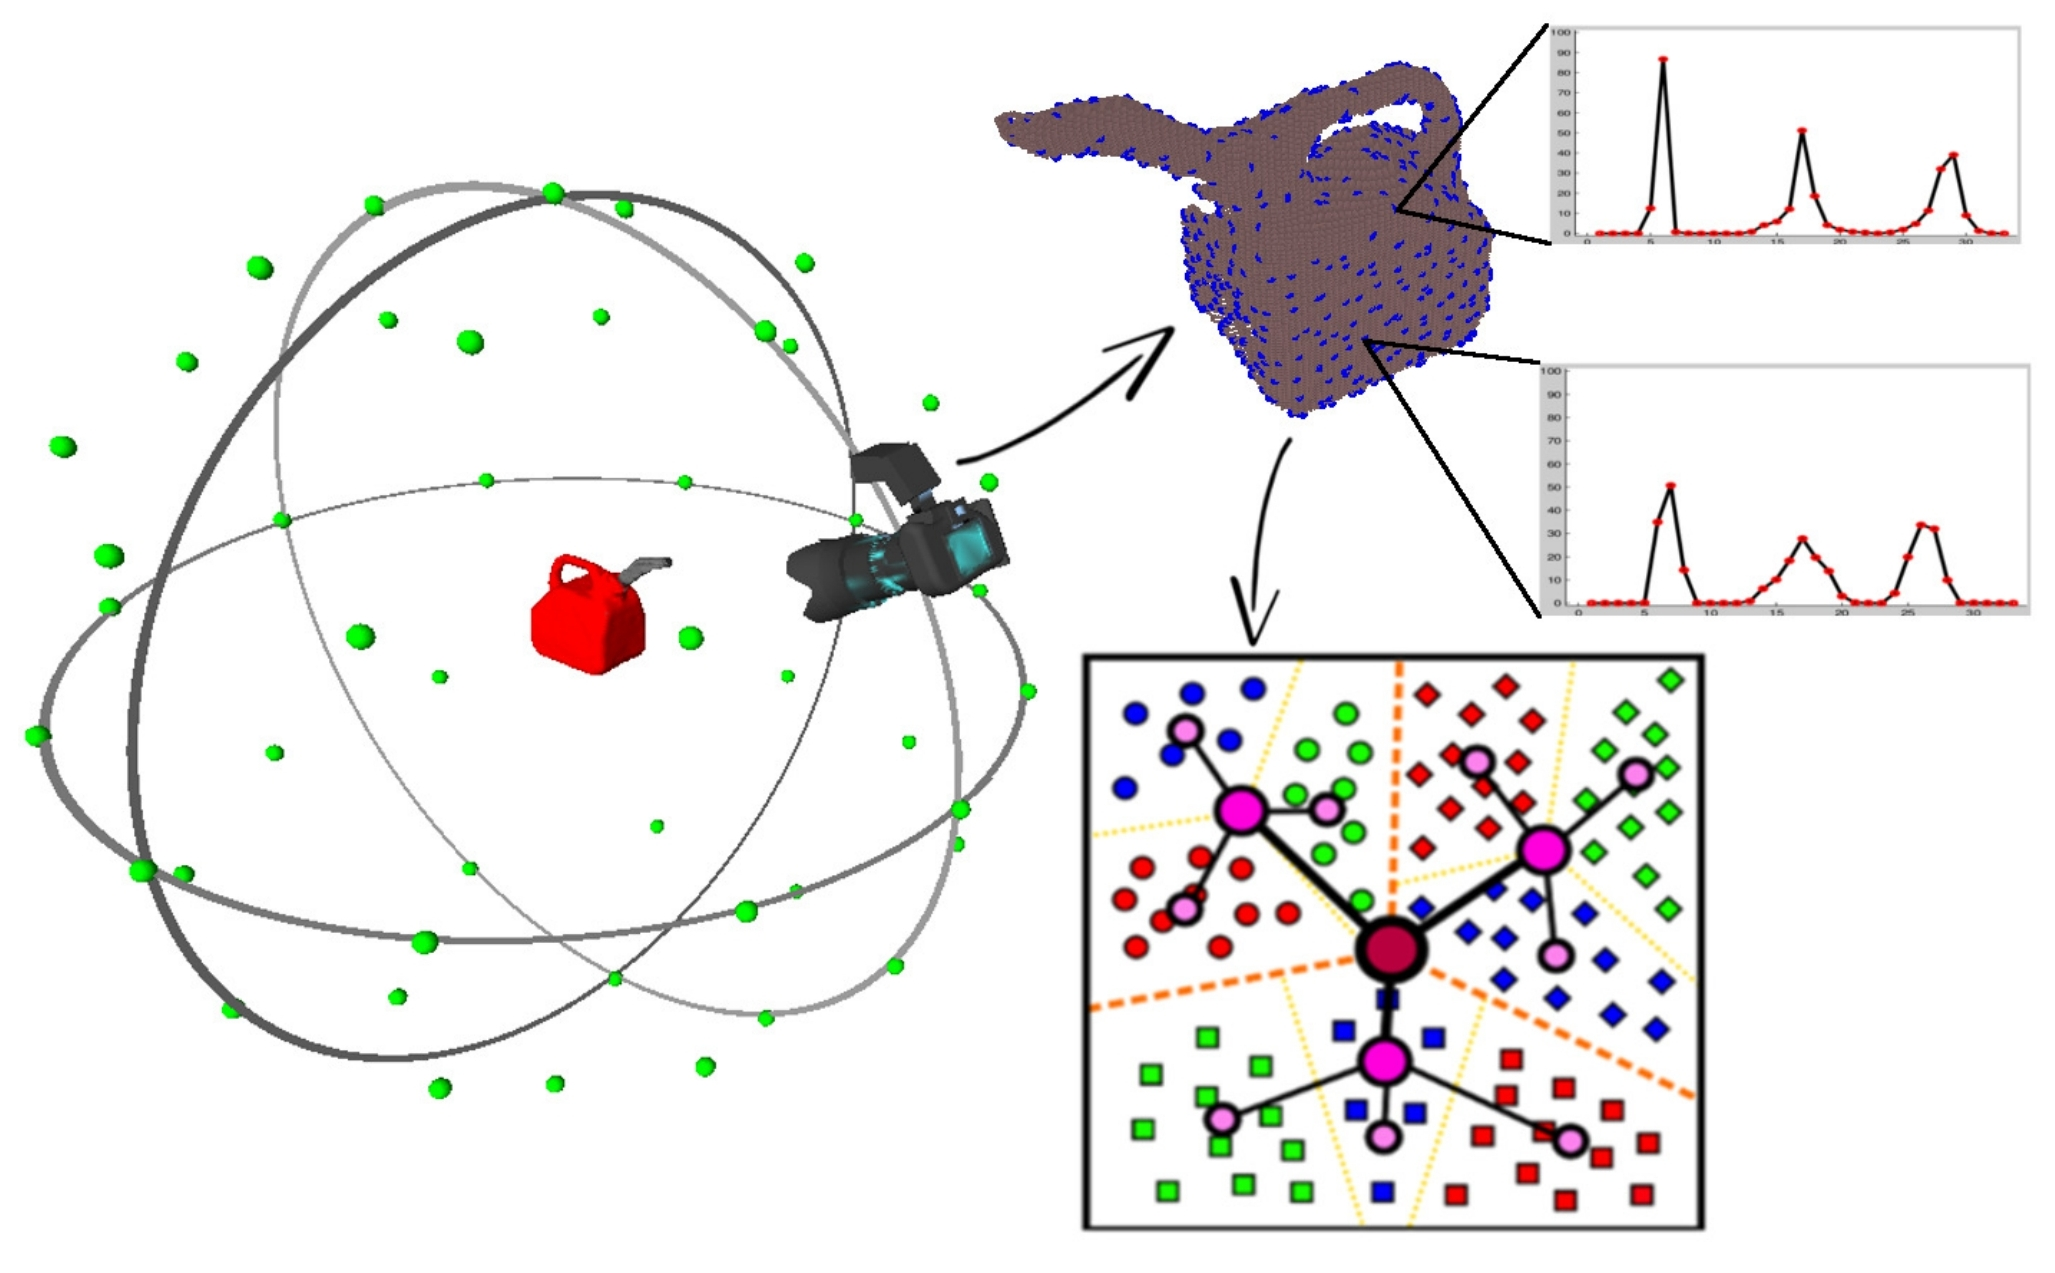
\includegraphics[scale=0.1]{atanasovmethod1_highres.jpg}
    \caption{ Figure taken from \cite{atanasov2014nonmyopic}.
  This figure illustrates the method of Atanasov et al. \cite{atanasov2014nonmyopic} which consists in allowing a camera to move on a sphere centered at the object location. The camera visits the desired viewpoints and obtains a corresponding point cloud for each one of them. Consequently, it ends up extracting relevant features as seen in the top right graph, which contribute to the construction of the VP-Tree in the bottom right corner. }
  
  \label{atanasovmethod1}
\end{figure}

\subsection{Learn-to-Score: Deep Learning approach}

Unlike the previous approach, which requires approximately solving a POMDP over a number of state transitions, Hepp et al. \cite{hepp2018learn} propose an alternative method using a trained Convolutional Neural Network (i.e. CNN). As expected, the heavy calculations are done during the training of the CNN, which allows the system to work very fast at test time, without any need for dynamic programming to calculate view utility. Moreover, this method is a greedy one, greedily selecting the next best view. Typically in the literature, an NBV method will be much like the one proposed by \cite{atanasov2014nonmyopic}, just that it will pick actions greedily instead of looking at the long term reward. This CNN approach stands out because it works well for very big landscapes and offers promising results for unmanned air vehicle/UAV applications like drones, quadrocopters and the like. Figure \ref{heppmethod1} shows the structure of the CNN. The authors train the network using simulated data, just like \cite{atanasov2014nonmyopic} do and prove that the encoded knowledge is transferable to real world scenes as well. A very interesting detail is that the training is done on a very peculiar dataset named: "Washington2" (see \cite{zamir2016generic}), but oddly enough, the network generalizes very well to all sorts of datasets, significantly different in their patterns of building height, distribution and geometry (ex: "SanFrancisco" dataset (from the broader \cite{zamir2016generic} dataset) with landscape from San Francisco USA, which is notorious for being unlike any other city in the world).  
\begin{figure}[t!]
  
  \centering
    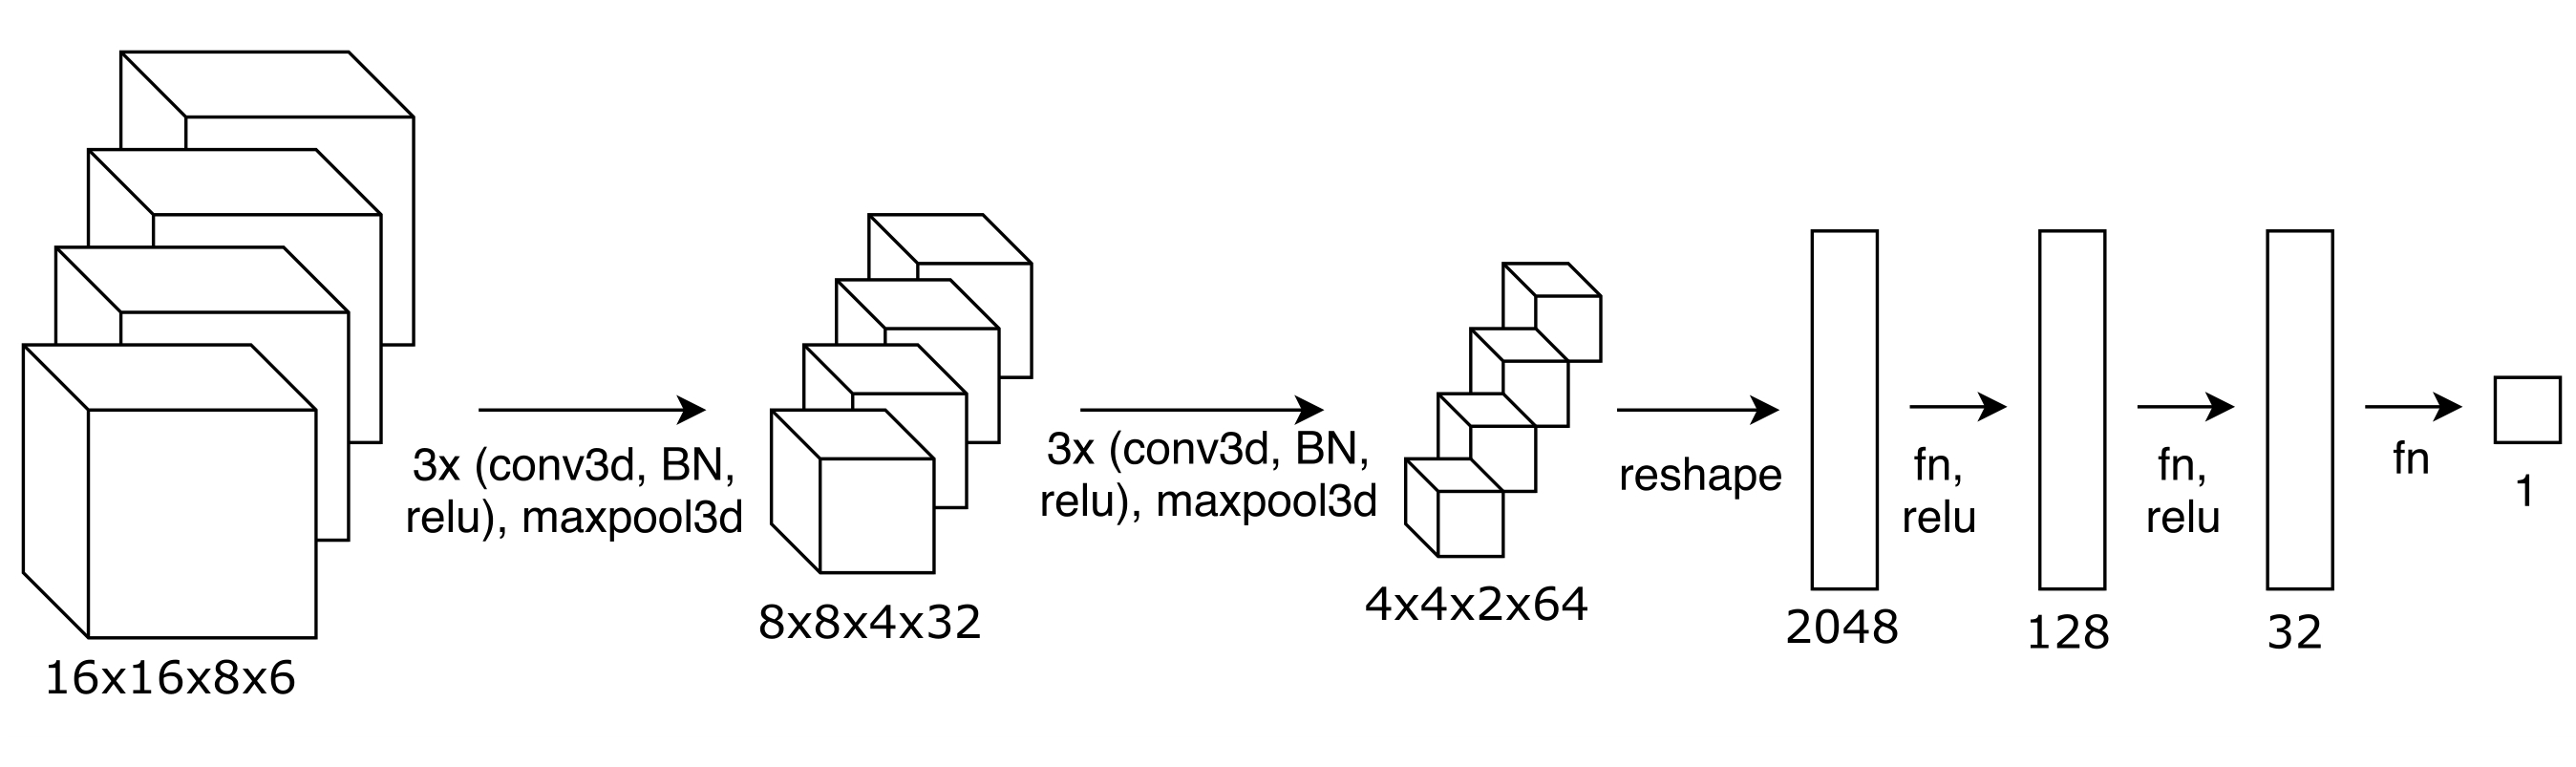
\includegraphics[scale=0.13]{heppmethod1_highres.jpg}
    \caption{Figure taken from \cite{hepp2018learn}.
  This figure illustrates the method of Hepp et al. \cite{hepp2018learn} which consists in using a CNN designed to approximate an oracle utility function. This approach is substantially different than a dynamic programming way of solving an MDP, which is the usual way in which active vision problems are posed.}
  \label{heppmethod1}
\end{figure}

The authors use an L2 loss function:
\begin{equation}
L(X,Y;\theta)=\sum_{n=1}^N \norm{f(X_i)-Y_i}^2 + \lambda \norm{\theta}^2
\end{equation}
 where $\theta$ are the model parameters and $(X_i, Y_i)$ are the input and output data points. More specifically: $X_i$  is the occupancy information and not the raw sensor data as one might initially assume, while $Y_i$ is the oracle's score as a numerical value. 


\subsection{Scheduling big sensor networks with real-time POMDPs}

One more interesting example that shows how a POMDP, although exponential in nature, can be greatly simplified with the right assumptions and solved in real time for practical applications is the one from Vaisenberg et al. \cite{vaisenberg2014scheduling}. They have been able to actuate a big system of cameras for surveillance purposes, such that they acquire important information about salient persons and actions. This can be useful for security reasons in airports or any crowded areas. The cameras can pan, zoom and tilt and they have the purpose of taking high resolution images of peoples' faces who are of interest. Of course they can't just greedily zoom in at every face because then, the system won't extract useful information about moving entities and the statistics of their movement. In other more metaphorical words: the "dynamics" of the world would not be accurate, and this hinders future planning about when to pursue and when to refrain from taking greedy actions. Staying "UP", or zoomed out is also important even though it implies lower detail images, because it allows the algorithm to extract important semantics about the world itself and what might be of interest in the future. So the system tries to balance the need of some other applications of taking greedy actions and high detail images, and its own need of knowing the world so that it can act greedily at the right time. In a way, it is a flavour of the exploration-exploitation dilemma. Since the intention is to use many cameras, in the order of tens, possibly hundreds, and each camera has many regions in its field of view that it can zoom into, the POMDP would therefore be intractable. Hence, the authors took some precautionary, simplifying measures and assumptions: the cameras have non-overlapping views (see Figure \ref{vaisenbergcameras}) and the background algorithms extract semantics from the environment in the form of correlations (see Figure \ref{vaisenbergcorrelation}). The way the cameras are placed spatially is such that a moving entity captured by one camera would correlate with the same entity being captured by another camera at a later point in time. Other cameras however, probabilistically "know" in advance that they won't see the entity until some later point in time, because they might be uncorrelated with the camera that observes the entity currently. As a result, the system now can trim a lot of branches and nodes in the decision tree that are not of interest.

\begin{figure}[t!]
  
  \centering
    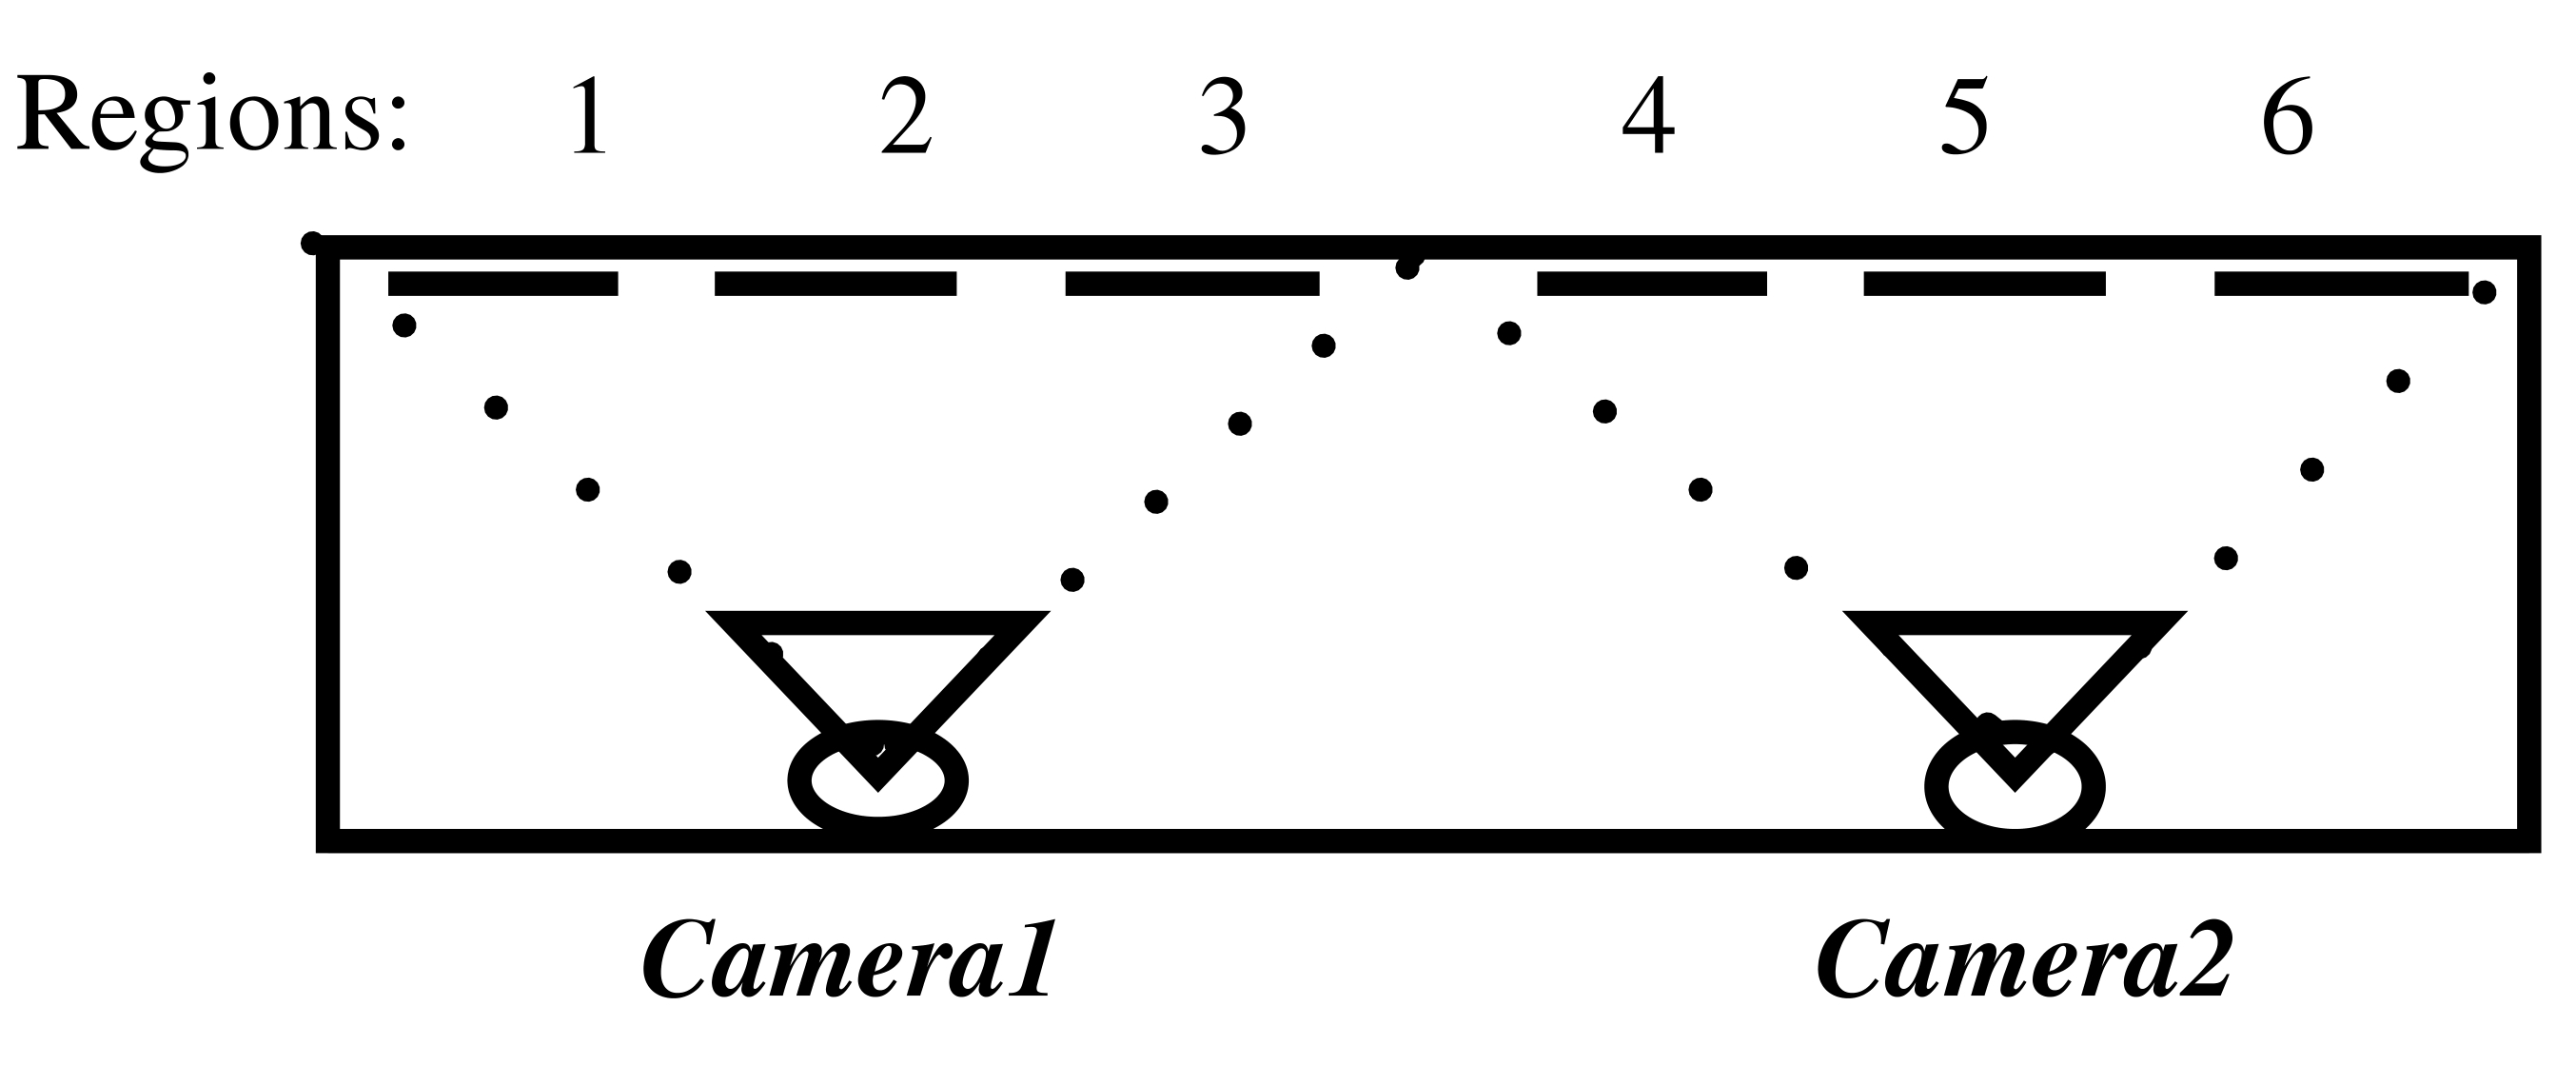
\includegraphics[scale=0.1]{vaisenbergmethod1_highres.jpg}
    \caption{ Figure taken from \cite{vaisenberg2014scheduling}.
  Long hallway continuously covered by cameras with non-overlapping fields of view as a simplifying assumption.}
  \label{vaisenbergcameras}
\end{figure}

\begin{figure}[t!]
  
  \centering
    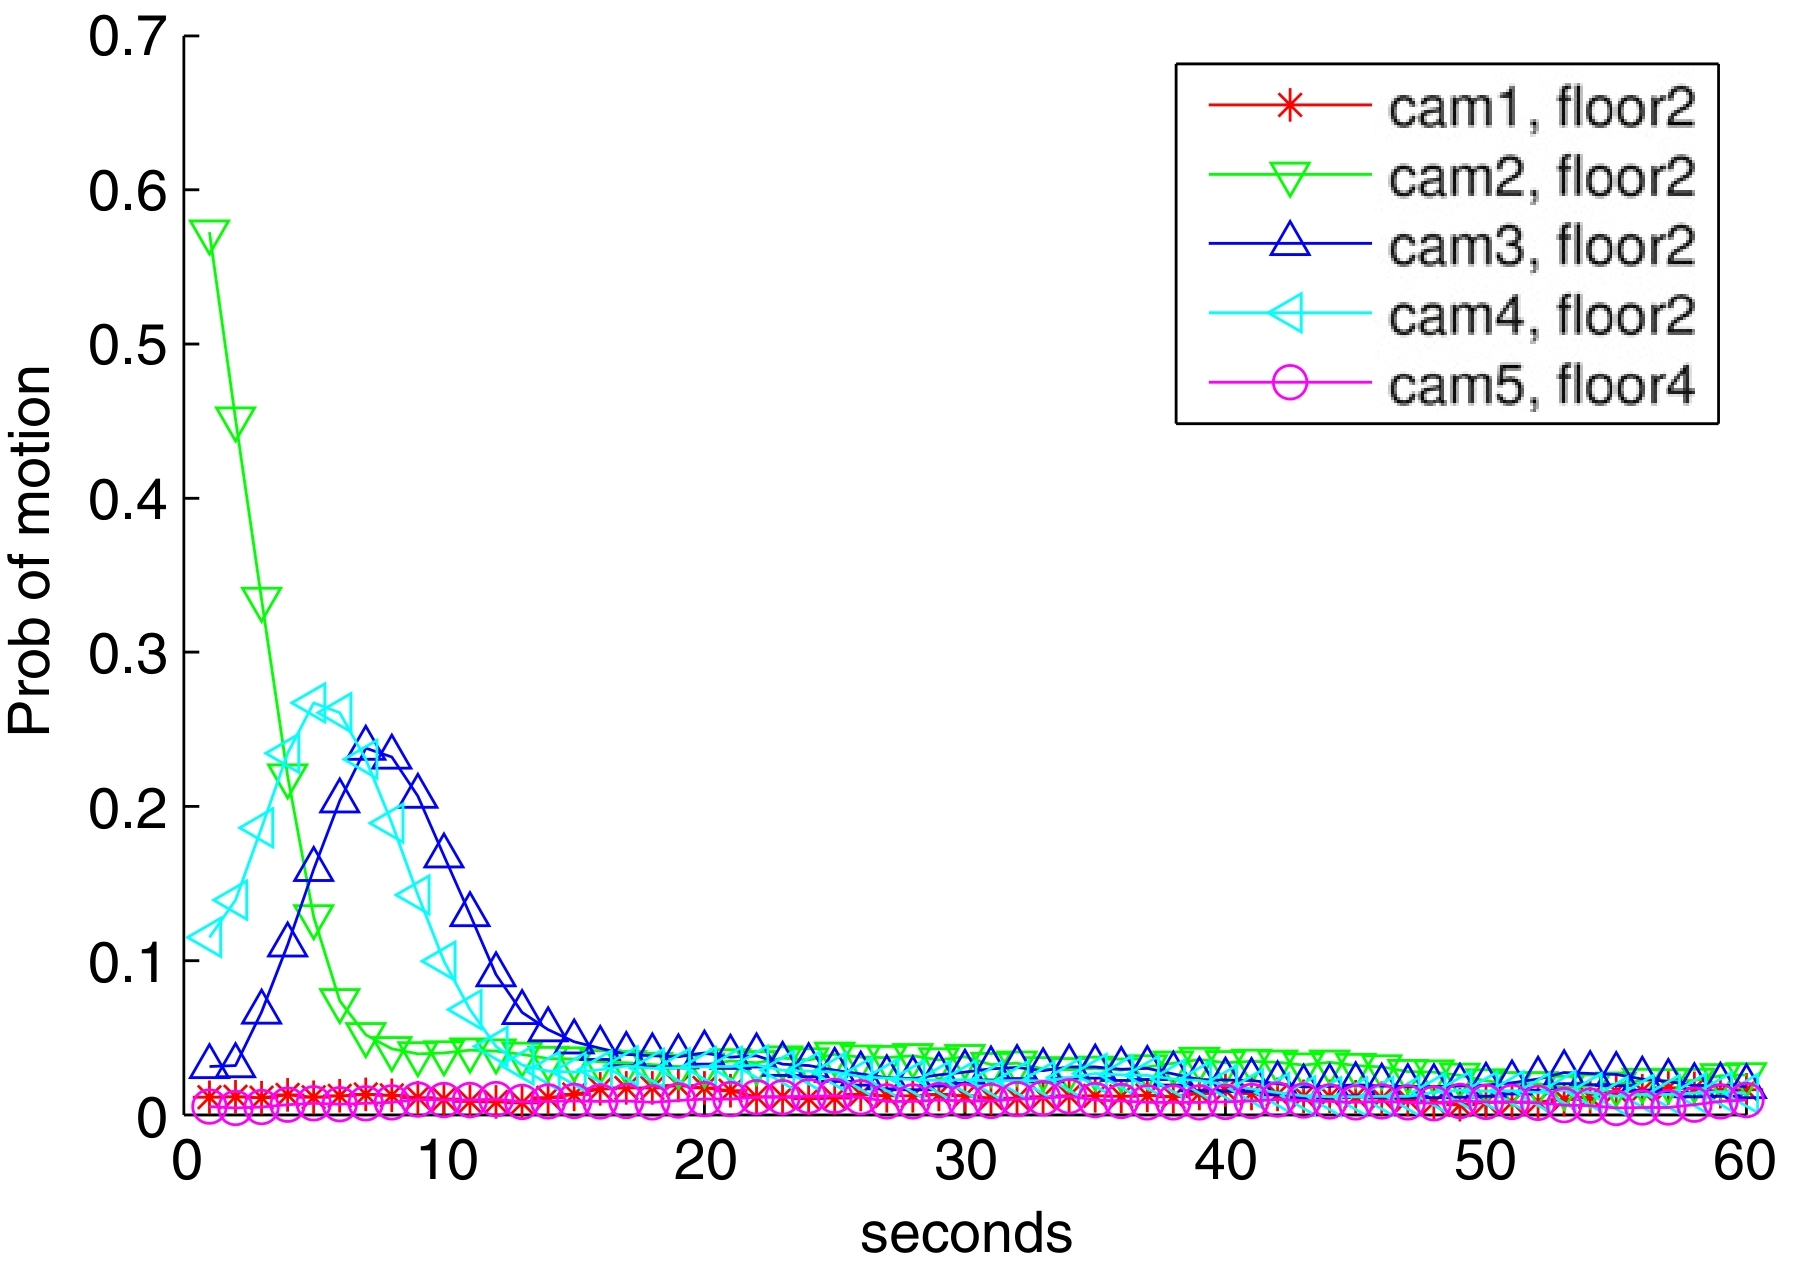
\includegraphics[scale=0.15]{vaisenbergmethod2_highres.jpg}
    \caption{ Figure taken from \cite{vaisenberg2014scheduling}.
  This figure illustrates the procedure of correlating camera data in order to predict what certain cameras will see in the future based on what other cameras observe currently. According to Vaisenberg et al. \cite{vaisenberg2014scheduling} this allows to significantly reduce the state space for the POMDP.}
  \label{vaisenbergcorrelation}
\end{figure}

Having described the 3 methods above, the next chapter will show the results and performance they exhibit in simulation and in practice.



\section{Experimental result and evaluation}




\subsection{Nonmyopic View Planning}



For the object classification and pose estimation approach, the authors try to compare it with 3 other solutions:
\begin{itemize}
\item \textbf{Greedy Mutual Information}: greedily maximize the mutual information function.
\item \textbf{Random Method}: random walk on the viewsphere while not revisiting the same viewpoints.
\item \textbf{Static Method}: take a single measurement at the initial position and decide based on that greedily. 
\end{itemize}

As Table \ref{tbl:atanasovsimevaluation1} shows, the classification is done correctly and with high confidence as well. However, note that the results are not much higher than the well established Greedy Mutual Information approach. The authors acknowledge this and say that the intention of their method is to have a more robust stopping criterion, i.e. adaptively decide when it makes sense to stop taking measurements based on the observations received online. 

\begin{table}[t!]
  \caption{Simulation \textbf{Accuracy} Results (created based on data from \cite{atanasov2014nonmyopic})}
  \label{tbl:atanasovsimevaluation1}
	\begin{adjustbox}{width=\columnwidth,center}
     \begin{tabular}{|l|l|l|l|l|l|l|l|}
     \hline
   Hypothesis & H(0$^\circ$)& H(60$^\circ$) & H(120$^\circ$) & H(180$^\circ$) & H(240$^\circ$) & H(300$^\circ$) & H(Other)\\
   \hline
  Static method & 60.35 & 53.90 & 51.49 & 49.13 & 56.11 & 54.29 & 89.87 \\


  Random method & 73.78 & 70.34 & 70.75 & 66.97 & 68.76 & 71.85 & 92.33 \\


  Greedy MI method & 82.63 & 80.14 & 76.93 & 75.60 & 75.29 & 81.78 & 94.65 \\


  \textbf{NVP method} & 87.98 & 83.78 & 82.81 & 82.61 & 78.73 & 81.60 & 93.20 \\
\hline
	
\end{tabular}  
\end{adjustbox} 
  
  %\includegraphics[width=\linewidth]{atanasovevaluation1_highres.png}
\end{table}

Since all the main experiments and training were done in simulations, the authors also show that the results are transferable to real world practical applications using a PR2 robot (see Table \ref{tbl:atanasovrealevaluation2}). 

\begin{table}[t!]
  \caption{Real-World \textbf{Accuracy} Results (created based on data from \cite{atanasov2014nonmyopic})}
  \label{tbl:atanasovrealevaluation2}
  \begin{adjustbox}{width=\columnwidth,center}
  \begin{tabular}{|l|l|l|l|l|l|l|l|}
  \hline
   Hypothesis & H(0$^\circ$)& H(60$^\circ$) & H(120$^\circ$) & H(180$^\circ$) & H(240$^\circ$) & H(300$^\circ$) & H(Other)\\
   \hline
  \textbf{NVP} Accuracy & 87.5 & 80.0 & 72.5 & 70.0 & 75.0 & 72.5 & 98.05 \\
  \hline
\end{tabular}
\end{adjustbox}
  %\includegraphics[width=\linewidth]{atanasovevaluation2_highres.png}
\end{table}





\subsection{Learn-to-Score: Deep Learning approach}


Regarding the CNN attempt to approximate a ground truth oracle function, Table \ref{tab:hepptable1} shows that it indeed manages to outperform significantly some of the most prominent hand-crafted solutions out there. Not only the score is accurate, but the decision time is better as Table \ref{tab:hepptable2} points out. These results one more time convince us of the efficiency of neural nets over vanilla methods in computer vision. However, there are certain trade-offs that will be discussed in the future section.
\begin{table}[t!]
\caption{\label{tab:hepptable1} Table refactored from \cite{hepp2018learn}. Efficiency Metric of the CNN utility function on the \textit{3D Street View} dataset \cite{zamir2016generic}, which contains models of different cities. As it can be observed, although the other functions are hand-crafted, trying to approximate a ground truth oracle is more effective.}
\begin{adjustbox}{width=\columnwidth,center}
\begin{tabular}{ |c|c|c|c|c|c| } 
\hline 
 Efficiency Metric & Washington2 & Washington1 & Paris & SanFrancisco & Neighborhood\\
 \hline
 Frontier & 0.40 & 0.29 & 0.57 & 0.09 & 0.27 \\ 
 AverageEntropy \cite{isler2016information}& 0.26 & 0.36 & 0.32 & 0.30 & 0.50 \\ 
 ProximityCount \cite{isler2016information}& 0.52 & 0.47 & 0.37 & 0.23 & 0.60 \\ 
 \textbf{CNN \cite{hepp2018learn}} & \textbf{0.91} & \textbf{0.88} & \textbf{0.87} & \textbf{0.77} & \textbf{0.74} \\
 Oracle (GT access) & 1.00 & 1.00 & 1.00 & 1.00 & 1.00 \\
 \hline
\end{tabular}
\end{adjustbox}

\end{table}

\begin{table}[t!]
\caption{\label{tab:hepptable2} Table refactored from \cite{hepp2018learn}. One of the advantages of not using an online dynamic programming approach is the lightning fast response time, in this case equal to the inference time of the neural network.}
\begin{adjustbox}{width=\columnwidth,center}
\begin{tabular}{ |c|c|c|c|c| } 
\hline
& Frontier & ProximityCount & AverageEntropy & CNN \cite{hepp2018learn}\\
\hline
Time in s & 0.61 & 5.89 & 8.35 & \textbf{0.57}\\
\hline
\end{tabular}
\end{adjustbox}

\end{table}








\subsection{Scheduling big sensor networks with real-time POMDPs}


Continuing with the last surveillance system in the above chapter, it can be observed in Figure \ref{vaisenbergevaluation1} that it indeed performs very well in terms of latency, with a very big number of cameras K. For a non-approximated solution, even a size of 10 to 30 would already be a big problem for real time operation. Figure \ref{vaisenbergevaluation2} illustrates that this is indeed the case, and note that the exact solution there, using an exhaustive tree search, only considers a depth of 2 seconds look-ahead to calculate the utility score. If a bigger depth of the tree would be considered, the latency would have a huge increase.
\begin{figure}[t!]
  
  \centering
    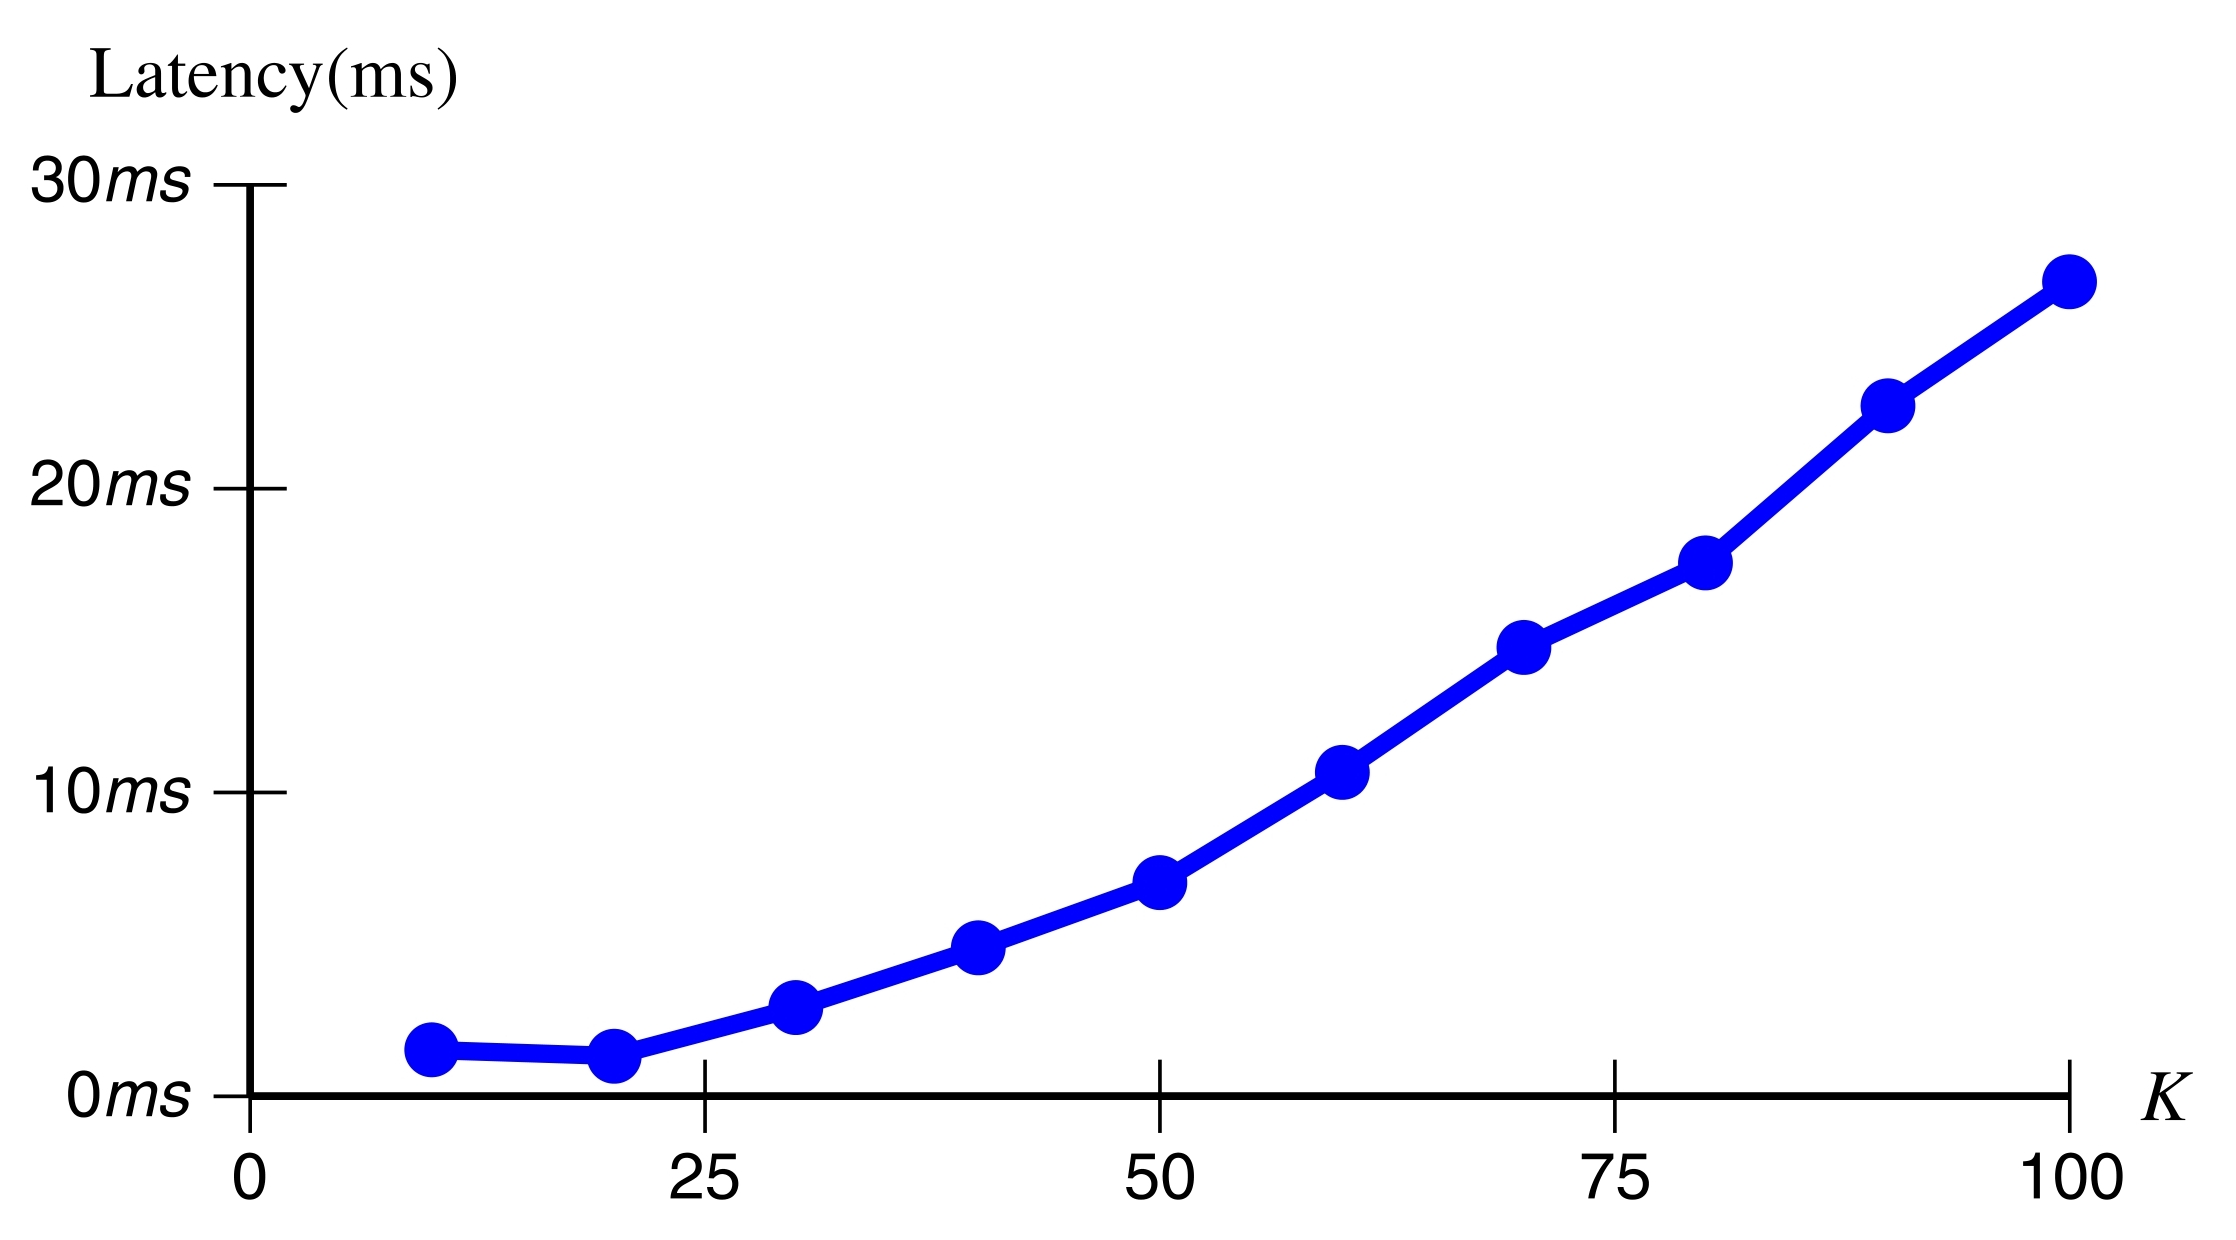
\includegraphics[scale=0.13]{vaisenbergevaluation1_highres.jpg}
    \caption{Figure taken from \cite{vaisenberg2014scheduling}. Using global semantics and local lookup tables, Vaisenberg et al. \cite{vaisenberg2014scheduling} have been able to achieve real-time performance using a very impressive number of cameras \textbf{\textit{K}}. As it can be seen, the marginal cost of adding one more camera is very small and does not increase the latency beyond what can be considered as real-time.}
  \label{vaisenbergevaluation1}
\end{figure}

\begin{figure}[t!]
  
  \centering
    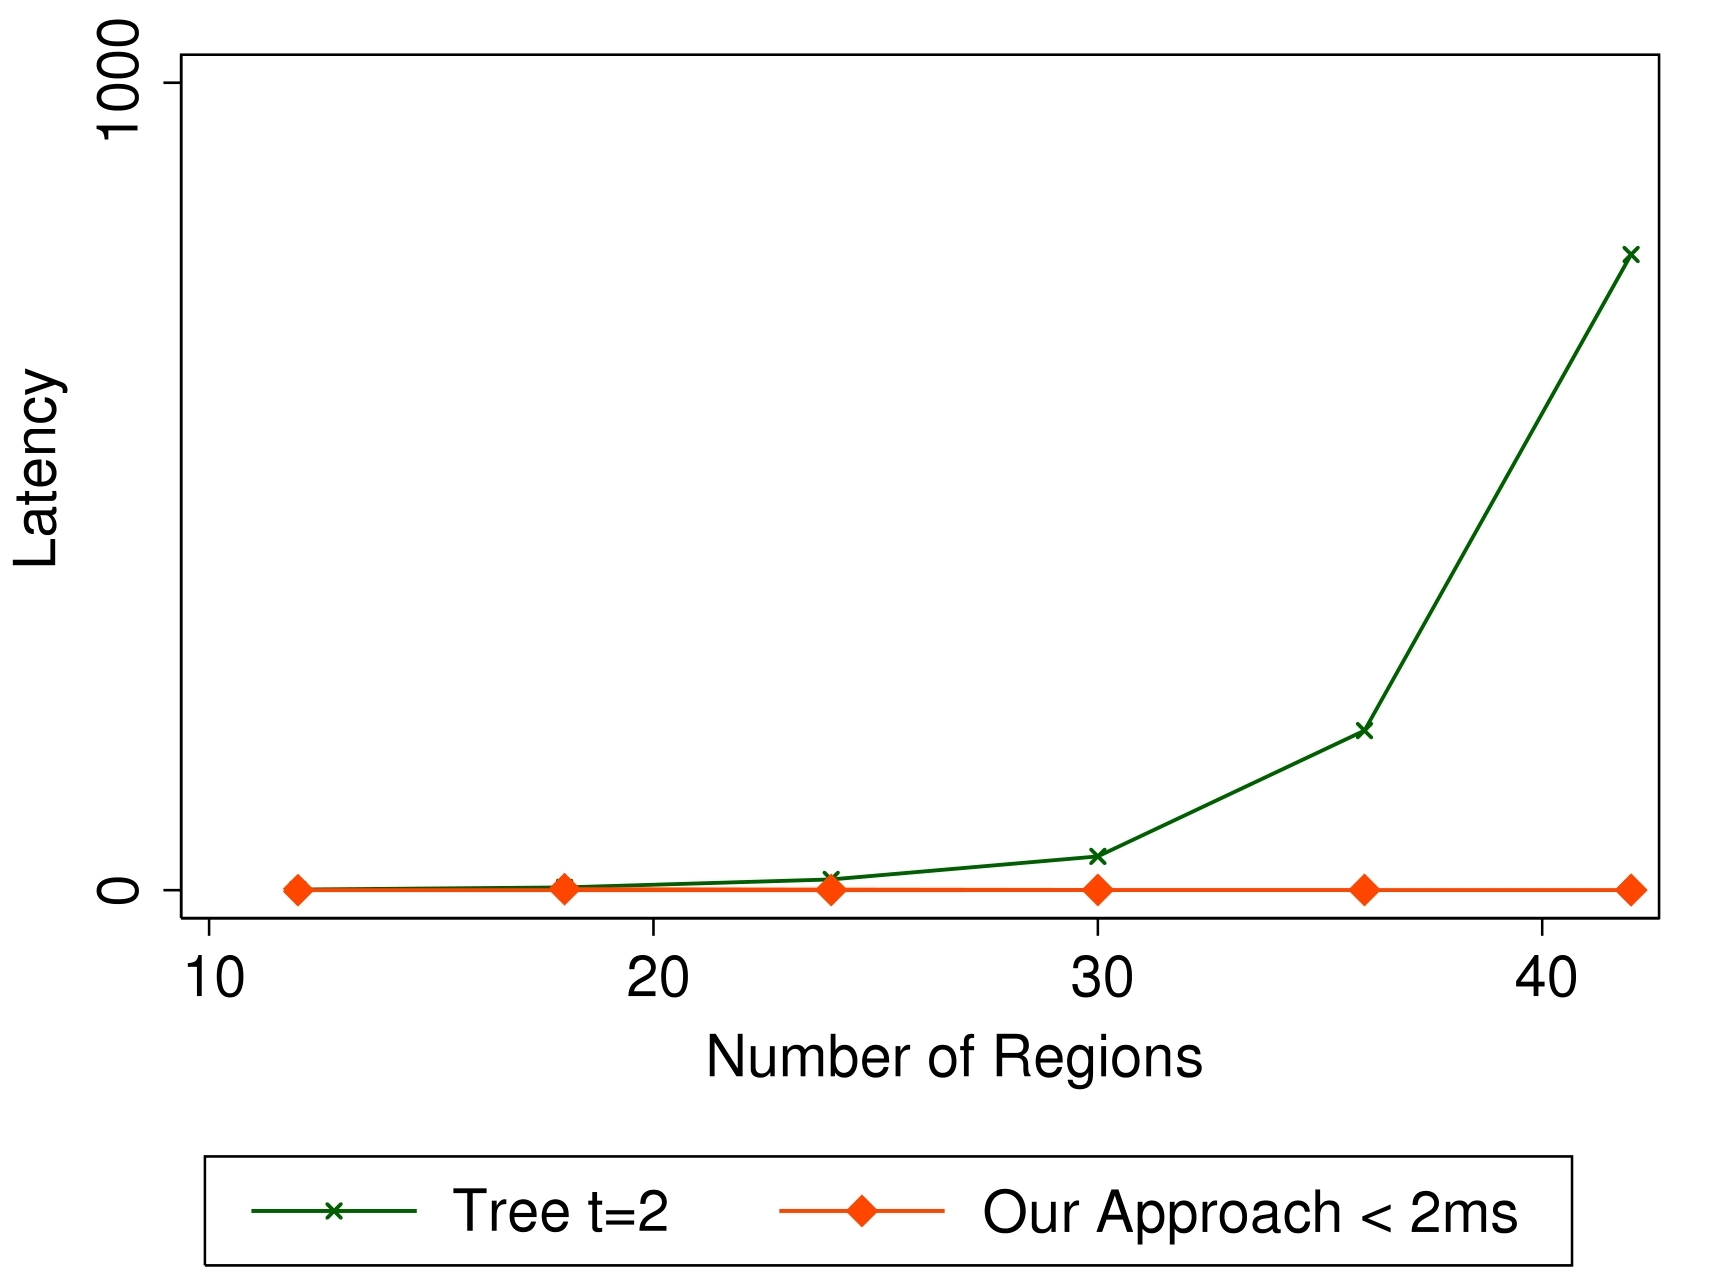
\includegraphics[scale=0.15]{vaisenbergevaluation2_highres.jpg}
    \caption{Figure taken from \cite{vaisenberg2014scheduling}.
  This figure motivates the need for approximating the solution of the POMDP using the method of Vaisenberg et al. \cite{vaisenberg2014scheduling}. Otherwise, the exact solution requires exponential computation time with each new added camera/region to monitor, and the solution cannot be considered real-time anymore.}
  \label{vaisenbergevaluation2}
\end{figure}













Considering these results, we will discuss the advantages and disadvantages in the following chapter and reason about when might one consider a certain approach over another.

\section{Discussion} % (fold)

In this section we will discuss the strengths and weaknesses of the already presented methods.

The method of Atanasov et al. \cite{atanasov2014nonmyopic} has the advantage that it tackles two aspects of computer vision which are very useful for practical applications: detection and pose estimation. Bridging the gap between these two problems would significantly contribute to solving the grasping problem in robotics. The disadvantage is that, although the results are promising and resemble the best ones from other methods, the authors did not factor in the problem of segmentation. All simulations are carefully constructed with objects on a table, in such a way that they do not require complex segmentation. It was not the scope of the work to create a customized segmentation component, but one can argue that it is a good way to reduce the complexity of the POMDP and obtain a more complete and practical system.

The CNN approach on the other hand, is very oriented towards solving practical issues. The authors argue that all POMDP approaches can only work for small scale problems and therefore, in order to be able to explore huge landscape, one needs a new way to tackle the problem, which is a trained neural net. What can be mentioned is that the CNN will try to approximate an oracle function, which knows the true utility score of a view, and the resulting function will presumably not have the exact theoretical guarantees as a handcrafted utility function might have (or as the true oracle has). However, as it was seen in the evaluation section, in practice, even without those theoretical proofs, the neural net performs better than well established methods and heuristic functions. A potential drawback is that there can always be some edge case that is not sufficiently addressed and different training experiments of the CNN would result in different behaviours, since the training process is stochastic by nature. A hand-crafted function is by definition more stable in its behaviour, at least until scientists will prove more things about neural nets and shed more light on the "black box" aspect that they are stigmatized with.

The third system, aiming to create a framework backbone on top of which many applications can run, tries to combine the best of both worlds:
\begin{itemize}
\item Make a system that can scale
\item Still use a POMDP to control the sensors
\end{itemize}

A huge advantage is that their sensor-correlation model is real time for large state spaces. The authors manage to find important simplifying aspects of the problem. However, this means that the model will only work for specialized environments and tasks, in this case: a people surveillance task. Many other problems however might not fulfil the underlying prerequisites to be modelled in a similar fashion. And since people surveillance might trigger ethical concerns, the reader will be positively surprised and rest-assured that the same correlation model can be applied to traffic lights control for the purpose of reducing traffic jam amongst other things.

\section{Conclusion}
In conclusion, what can be said about active perception is that it is a field with a lot of potential applications, that is currently receiving a lot of attention from the research community. Up until recently it was considered a niche topic within the computer vision realm, but things have changed with the advent of cheaper, high-quality sensing devices. The POMDP approach, since it is considered a PSPACE-complete problem (see \cite{papadimitriou1987complexity} and \cite{arora2009computational}), means that approximated solutions will be developed for concrete tasks of active perception, on a case by case basis. In other words, there will not be a one fits all solution, till the time when POMDPs are theoretically solved, if this ever happens. Other solutions like neural nets and various efficient data structures and clever algorithmic tricks will always remain an option and that is what makes the field so reach, interesting, diverse and creative from an engineering point of view. We convinced ourselves of the richness of applications and diversity of solutions throughout the chapters. There is more work to be done however, especially in the decentralized POMDP domain, where things are still in their infancy in both theoretical as well as practical terms.

\newpage
\bibliographystyle{unsrt}
\bibliography{bib}



\end{document}
